\chapter[Gerenciamento dos Riscos]{Gerenciamento dos Riscos}

O plano de riscos é a área que visa aumentar as taxas de sucesso de um projeto, visto que este é responsável pela gerência dos riscos identificados, apontando seus impactos e como mitigá-los \textbf{(\cite{pmbok2004})}.

Riscos são eventos ou condições que se ocorrerem podem afetar o projeto positivo ou negativamente, afetando características do projeto como escopo, tempo, custo, qualidade entre outros. Devido aos impactos prejudiciais que os riscos podem gerar quanto oportunidades, surge a necessidade de gerenciar os mesmo, para que a resposta a esses eventos sejam de forma planejada e eficiente, a fim de garantir o sucesso do projeto.

Devido a natureza dos riscos e seus impactos sobre o projeto, estes precisam ser analisados depois de identificados. Para isso, foram definidos três atributos para os riscos: Probabilidade, impacto e interesse. 

A chance está relacionado com a probabilidade do risco acontecer. É definida em três níveis: Baixa, Média e Alta probabilidade de acontecer.

O impacto está relacionado ao quanto este risco irá afetar o projeto, principalmente com relação a questões de escopo, tempo, custo e sucesso do projeto. O impacto é definido em três níveis: Baixo, Médio e Alto impacto no projeto.

O interesse é o produto de uma relação dos outros dois, onde baseado nas chances de acontecer e no impacto do risco será estipulado um interesse da organização com esse risco. Também é definido em três níveis: Baixo, Médio e Alto interesse no risco, de acordo com a matriz seguinte:

\begin{figure}[!ht]
\centering
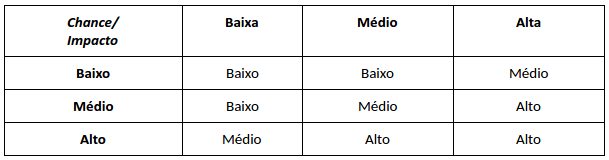
\includegraphics[scale=0.4, angle = 360]{figuras/risco1}
\caption{Matriz de interesses do risco (fonte: Autor)}
\label{Matriz de interesses do risco (fonte: Autor)}
\end{figure}
\FloatBarrier

Deve-se notar que dado a natureza do projeto e seus integrantes, essas chances serão estimadas baseadas em experiência dos integrantes, com um menor rigor metodológico que poderia ser exigido para essas estimações.	

O projeto proposto utiliza a estratégia descrita na metodologia utilizada \cite{pmbok2004} para a construção do plano de riscos. Os riscos identificados foram descritos na tabela abaixo

\begin{figure}[!ht]
\centering
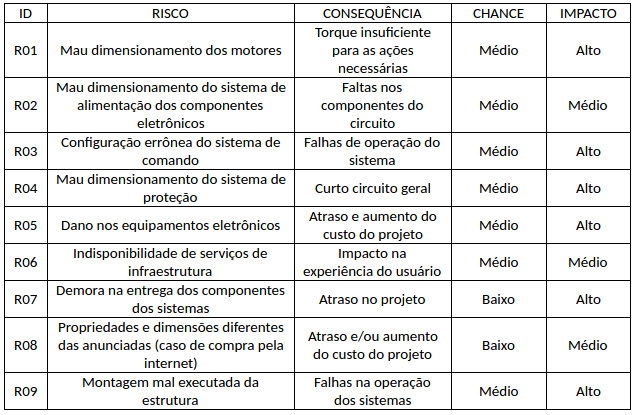
\includegraphics[scale=0.4, angle = 360]{figuras/risco2}
\caption{Riscos do Projeto (fonte: Autor)}
\label{Riscos do Projeto (fonte: Autor)}
\end{figure}
\FloatBarrier

Utilizando a matriz de Chance X Impacto, nós podemos definir o interesse da equipe naquele risco e também listar a ação de mitigação para aquele risco.

\begin{figure}[!ht]
\centering
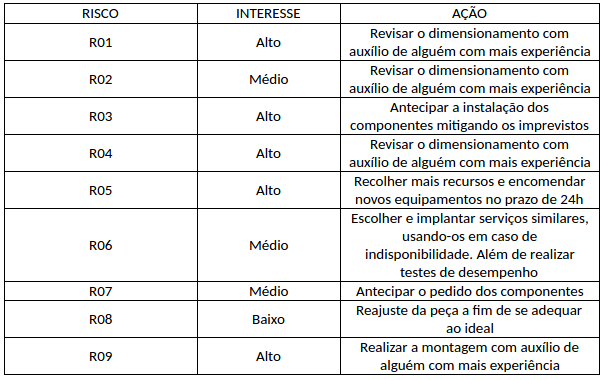
\includegraphics[scale=0.4, angle = 360]{figuras/risco3}
\caption{Interesse e Mitigação dos riscos (fonte: Autor)}
\label{Interesse e Mitigação dos riscos (fonte: Autor)}
\end{figure}
\FloatBarrier
